\documentclass[journal,12pt,twocolumn]{IEEEtran}
\usepackage{graphicx}
\graphicspath{{./figs/}}{}
\usepackage{amsmath,amssymb,amsfonts,amsthm}
\newcommand{\myvec}[1]{\ensuremath{\begin{pmatrix}#1\end{pmatrix}}}
\usepackage{listings}
\usepackage{watermark}
\usepackage{titlesec}
\let\vec\mathbf
\lstset{
frame=single, 
breaklines=true,
columns=fullflexible
}
\thiswatermark{\centering \put(0,-105.0){
\includegraphics[scale=0.15]{/sdcard/IITH/matrix/line/figs/logo.png}} }

\title{\mytitle}
\title{
Matrix Assignment - Lines
}
\author{Surajit Sarkar}
\begin{document}
\maketitle
\tableofcontents
\bigskip


\section{\textbf{Problem}}
One side of a rectangle lies along the line 4x+7y+5=0.
Two of its vertices are (-3,1) and (1,1).Find the equation of the other sides.


\section{\textbf{Solution}}
given
\begin{align}
     \Vec{A}&=\myvec{-3\\1}\\
     \Vec{C}&=\myvec{1\\1}
\end{align}
The direction of given line
\begin{align}
  4\vec{x}&+7\vec{y}+5=0\\
  \implies& 7\vec{y}=-4\vec{x}-5\\
  \implies& \vec{y}=\frac{-4}{7}\vec{x}-\frac{5}{7}\\
   \implies&\vec{L}=\vec{m}=\myvec{1\\{\frac{-4}{7}}}
\end{align}
The direction vector of line $\vec{AC}$ 
\begin{equation}
    d_{\vec{AC}}=\vec{A}-\vec{C}=\myvec{-4\\0}
\end{equation}
$\vec{AC}$ is diagonal of the given rectangle between $\vec{AC}$ and $\vec{AB}$
\\

where
\\
\begin{align}
    Cos\theta={\frac{\vec{m}^{\top}d_{\vec{AC}}}{\|\vec{m}\|\|\vec {m}_{\vec{AC}}\|}}
\end{align}
Vertices for $\vec{A}$ and $\vec{B}$
\begin{align}
    \vec{B}-\vec{A}&=R_{\theta}{\myvec{\vec{C}-\vec{A}}} {\frac{\myvec{\vec{A}-\vec{C}}Cos\theta}{\|\vec{A}-\vec{C}\|}}\\
    \vec{D}-\vec{A}&=R_{\frac{\pi}{2}-0}\myvec{\vec{C}-\vec{A}} Sin\theta
\end{align}
where
\begin{align}
    R=\myvec{Cos\theta&-Sin\theta\\Sin\theta&Cos\theta}
\end{align}
\\
\section{\textbf{Figure}}
\begin{figure}[h]
    \centering
    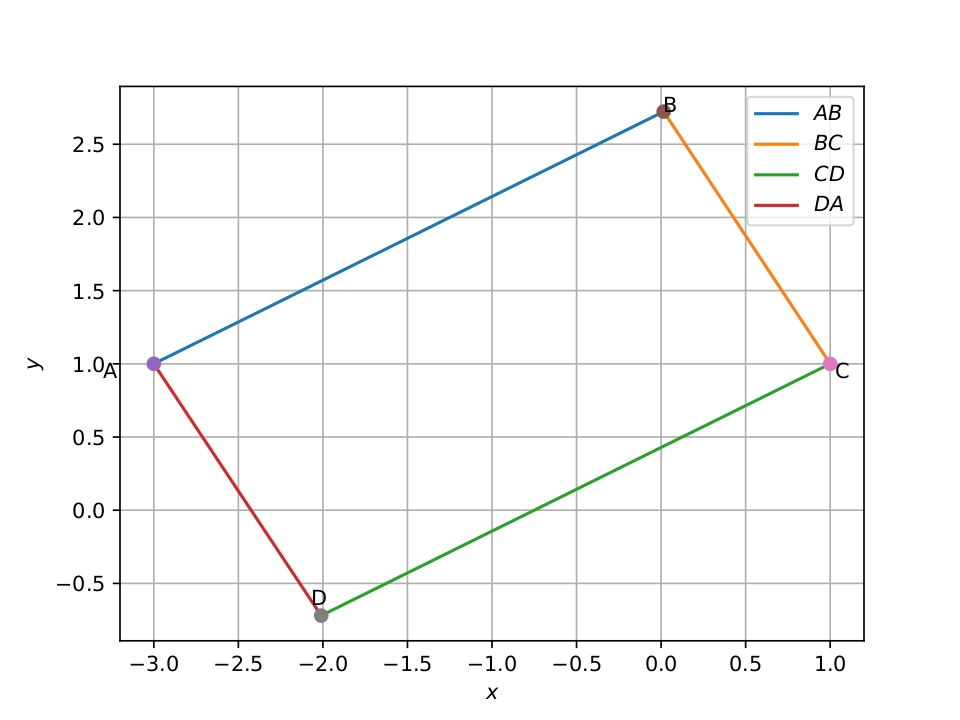
\includegraphics[width=\columnwidth]{/sdcard/IITH/matrix/line/figs/fig.jpg}
    \label{fig:my_label}
\end{figure}


\section{\textbf{Code Link}}

\begin{lstlisting}
https://github.com/sssurajit/fwc/blob/main/line/codes/line.py
\end{lstlisting}
Execute the code by using the command\\
\textbf{python3 line.py}
\end{document}
